\chapter{INTRODUCCIÓN}

En el Procesamiento Digital de Imágenes, la Mejora del Contraste es un proceso que consiste en la transformación de pixeles de una imagen, con la finalidad de realizar cambios de manera tal a resaltar uno o más objetos dentro de la imagen tratada. El objetivo principal del trabajo de Mejora del Contraste es obtener una nueva imagen cuyo Contraste sea más adecuado para la aplicación específica que se utilizará después \cite{gonzalez02a}.

La Mejora del Contraste es un paso de preprocesamiento fundamental para varias aplicaciones. En la Figura \ref{fig:casa1} se muestra un ejemplo que representa intuitivamente el efecto del proceso de Mejora de Contraste. Algunas de las aplicaciones que más se benefician de éste proceso se detallan a continuación:

\begin{itemize}
	\item Imágenes Médicas (como ejemplos es posible tomar: el Diagnóstico Asistido por Computadora \cite{doi2007computer}, Imágenes de Tomografía Computarizada \cite{doi:10.1056/NEJM199303113281008}, y otros).
	\item Sensoreamiento Remoto \cite{lillesand2014remote},

	\item Imágenes satelitales \cite{demirel2010satellite},

	\item Imágenes astronómicas \cite{doi:10.1080/00223638.1981.11738127},

	\item Imágenes biométricas\cite{bennet2011fingerprint},

	\item Otras\cite{BEGHDADI1989162}.
	
\end{itemize}



Las técnicas basadas en Ecualización del Histograma se mostraron extensivamente válidas para enfocar los problemas de Mejora del Contraste \cite{pizer1987adaptive,zuiderveld1994contrast,580378}. %\cite{Gonzalez02a,pizer1987adaptive,zuiderveld1994contrast,580378}. 
Varias Meta-Heurísticas en contextos de Optimización Mono-Objetivo, y también Optimización Multi-Objetivo fueron testeadas satisfactoriamente de manera a resolver problemas de Mejora del Contraste en imágenes en escala de gris \cite{morepso,more2015parameter,812529,HOSEINI2013879}. Sin embargo, la Optimización Multi-Objetivo aplicada a la Mejora del Contraste en imágenes a color supone dificultades adicionales, debido a que es necesario preservar la información de color presente dentro de dichas imágenes.

\begin{figure}[H]
\centering
    %\begin{subfigure}[t]{0.45\textwidth}
    \begin{subfigure}[Imagen Original]{
	    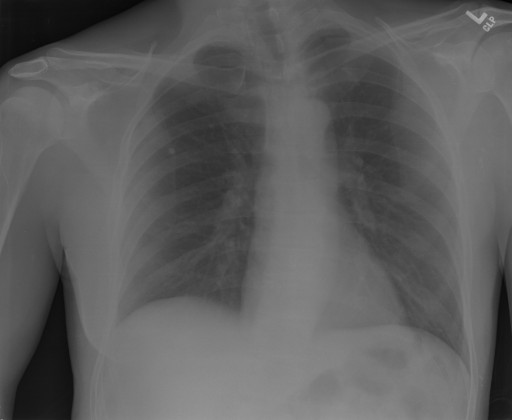
\includegraphics[width=0.4\linewidth,
	    keepaspectratio]{./Figures/chest.jpg}}
    %\caption{Original Image. $\mathscr{H_Y}=0.207231$, $SSIM_R=1$, $SSIM_G=1$, $SSIM_B=1$}
    \label{fig:casa1original}
    \end{subfigure}
     %add desired spacing between images, e. g. ~, \quad, \qquad, \hfill etc. 
      %(or a blank line to force the subfigure onto a new line)
    \begin{subfigure}[Imagen con contraste mejorado]{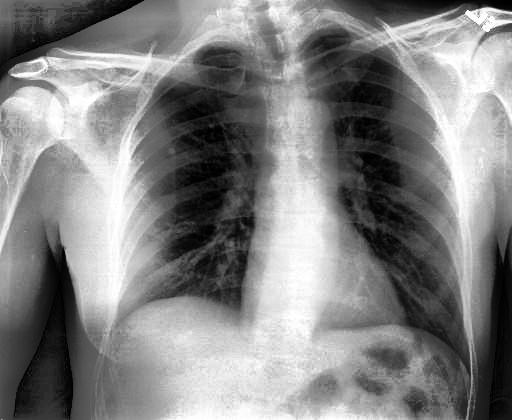
\includegraphics[width=0.4\linewidth,
	    keepaspectratio]{./Figures/chestclahe1.jpg}}
    %\begin{subfigure}[t]{0.45\textwidth}
    %\caption{Enhanced Image. $\mathscr{H_Y}=0.611275$, $SSIM_R=0.00897331$, $SSIM_G=0.00823064$, $SSIM_B=0.00851013$}
    \label{fig:casa1enhanced1}
    \end{subfigure}
    ~ %add desired spacing between images, e. g. ~, \quad, \qquad, \hfill etc. 
    %(or a blank line to force the subfigure onto a new line)
    \caption{En (a) se muestra una imagen en escala de grises con bajo contraste, y en (b) la misma imagen con contraste mejorado para una posterior utilización.}\label{fig:casa1}
    \end{figure}


    Ésta propuesta consiste en realizar pruebas de Mejora del Contraste con imágenes a color transformadas desde el espacio de colores $RGB$ al espacio de colores $YCbCr$ de manera a realizar la Mejora de Contraste basada en Optimización Multi-Objetivo. Contrast Limited Adaptive Histogram Equalization (CLAHE) se aplica sobre el canal $Y$ de la imagen de prueba, de manera a modificar el contraste, y la imagen resultante se transforma nuevamente a $RGB$ de forma a evaluar la Mejora del Contraste lograda, además de la similaridad entre canales de color.

%Our proposal consist in testing images transformed from $RGB$ color space to $YCbCr$ in order to perform MMO-based CE. Contrast Limited Adaptive Histogram Equialization (CLAHE) is applied over the $Y$ channel of the test image in order to modify contrast, and the resultant image is transformed back to $RGB$ in order to evaluate the similarity between color channels.

%The rest of the paper is organized as follows: in Section \ref{sec:theorethical_framework}, the fundametal concepts for this work are presented, in Section \ref{sec:proposal} the CE problem is posed, and our approach is presented, in Section \ref{sec:results_discussion} the results achieved are discussed in detail, and finally in \ref{sec:conclusion} some final points are remarked.


\section{Objetivos}
\subsection{Objetivo General}
Desarrollar un algoritmo de mejora de contraste para imágenes a color, utilizando un enfoque de Metaheurística Multi-Objetiva pura. El mismo debe de entrenar al algoritmo de Mejora del Contraste para la obtención de variables de decisión que logren mejorar el contraste de imágenes digitales. 
%Desarrollar un algoritmo de mejora de contraste para imágenes en escala de grises e imágenes en color que utiliza la matemática morfológica multiescala.
\subsection{Objetivos específicos}
\begin{itemize}

	\item Desarrollar un nuevo algoritmo de Mejora del Contraste de imágenes a color basado en Metaheurísticas Multi-Objetivo.

	\item Demostrar la factibilidad del enfoque de Mejora de Contraste de imágenes a color basado en Metaheurísticas Multi-Objetivo puras.

    \item Entrenar al algoritmo de Mejora del contraste para la obtención de variables de decisión para un conjunto de imágenes de prueba tipo.

	\item Encontrar alternativas de implementación que ayuden a subsanar problemas inherentes a los enfoques basados en Metaheurísticas Multi-Objetivo, cuando la cantidad de objetivos sobrepasa a tres.
% 	\item Proponer un nuevo algoritmo que utiliza matemática morfológica multiescala para la mejora del contraste de imágenes en escala de grises e imágenes en color.

% 	\item Comparar el algoritmo propuesto con algoritmos que modifican el histograma, tanto local como global, en imágenes en escala de grises.

% 	\item Comparar el algoritmo propuesto con un algoritmo que utiliza la transformada de top-hat en escalas múltiples en imágenes en escala de grises.

% 	\item Establecer relaciones de orden en los espacios de color RGB, HSI y HSV, de tal forma que el algoritmo propuesto sea aplicable a imágenes en color.

% 	\item Comparar el algoritmo propuesto con algoritmos que modifican el histograma, tanto local como global, en imágenes en color.

% 	\item Comparar el algoritmo propuesto con un algoritmo que utiliza la transformada de top-hat en escalas múltiples en imágenes en color.

% 	\item Comparar los tiempos de computo del algoritmo propuesto con un algoritmo que utiliza la transformada de top-hat en escalas múltiples.

\end{itemize}

\section{Estructura de la tesis}
El trabajo, en las secciones siguientes se organiza de la siguiente manera: en el capítulo \ref{sec:theorethical_framework}, los conceptos fundamentales de éste trabajo se presentan; en el capítulo \ref{sec:proposal} se presenta el problema de Mejora de Contraste, y el enfoque de éste trabajo se muestra; en el capítulo \ref{sec:results_discussion} se discute en detalle los resultados obtenidos, y finalmente en el capítulo \ref{sec:conclusion} se hacen algunos comentarios finales.
